% Hình: Khung Mixture of Experts (Mục 3.5)
% Gói: TikZ thuần (positioning + fit)
\documentclass[border=6pt]{standalone}
\usepackage[utf8]{vietnam}
\usepackage{amsmath,amssymb}
\usepackage{xcolor}
\usepackage{tikz}
\usetikzlibrary{positioning,fit,arrows.meta,calc,backgrounds}

\definecolor{qpurple}{HTML}{7E57C2}
\definecolor{qfill}{HTML}{ECE3F7}
\definecolor{slate}{HTML}{5B6470}
\definecolor{slatefill}{HTML}{EDEFF2}
\definecolor{lssorange}{HTML}{CF8A2A}
\definecolor{lssfill}{HTML}{FBE7C6}
\definecolor{inkdark}{HTML}{23272E}

\tikzset{
  >={Stealth[length=2.4mm]},
  every node/.style={font=\sffamily\small, text=inkdark},
  io/.style={draw=slate, rounded corners=2pt, thick, align=center, minimum height=8mm, minimum width=12mm},
  router/.style={draw=slate, fill=slatefill, rounded corners=2pt, thick, align=center, minimum height=8mm, minimum width=20mm},
  expert/.style={draw=qpurple, fill=qfill, rounded corners=2pt, thick, align=center, minimum height=8mm, minimum width=20mm},
  op/.style={draw=lssorange, fill=lssfill, circle, thick, inner sep=1pt, minimum size=6mm},
  flow/.style={-{Stealth[length=2.4mm]}, line width=0.9pt, draw=inkdark},
  gate/.style={-{Stealth[length=2mm]}, line width=0.8pt, draw=slate, dashed},
  lbl/.style={font=\sffamily\scriptsize, text=slate},
}

\begin{document}
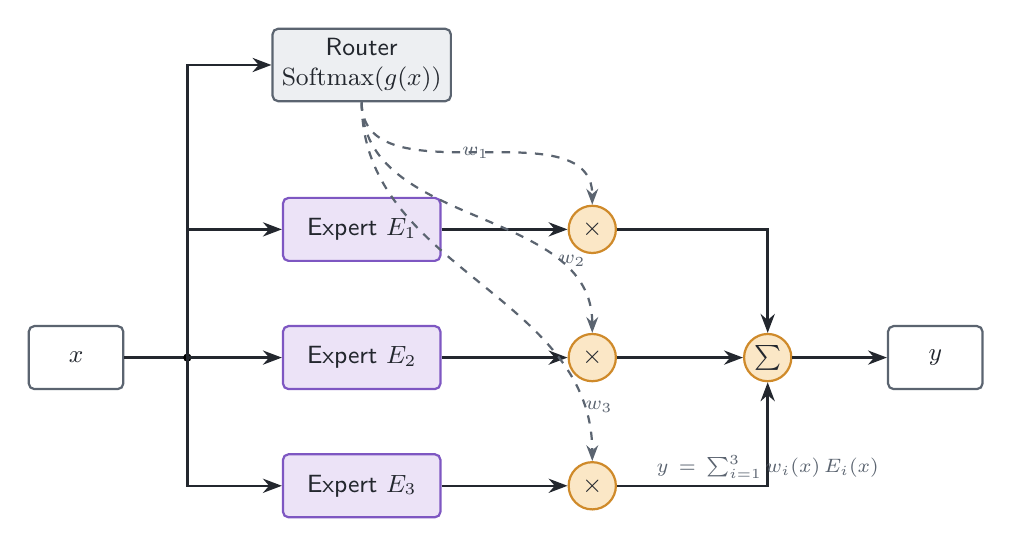
\begin{tikzpicture}
  % 1. CỘT ĐẦU VÀO
  \node[io] (x) {$x$};

  % 2. CỘT CHUYÊN GIA & ROUTER
  % Căn lề phải so với x, sắp xếp dọc
  \node[expert, right=20mm of x] (e2) {Expert $E_2$};
  \node[expert, above=8mm of e2] (e1) {Expert $E_1$};
  \node[expert, below=8mm of e2] (e3) {Expert $E_3$};
  
  % Router nằm chính giữa phía trên tập nhánh xử lý
  \node[router, above=12mm of e1] (router) {Router\\ $\mathrm{Softmax}(g(x))$};

  % 3. CỘT NHÂN TRỌNG SỐ (Multipliers)
  \node[op, right=16mm of e1] (m1) {$\times$};
  \node[op, right=16mm of e2] (m2) {$\times$};
  \node[op, right=16mm of e3] (m3) {$\times$};

  % 4. CỘT CỘNG GỘP & ĐẦU RA
  \node[op, right=16mm of m2] (sum) {$\sum$};
  \node[io, right=12mm of sum] (y) {$y$};

  % ==========================================
  % VẼ ĐƯỜNG DẪN DỮ LIỆU (DATA FLOW)
  % ==========================================
  
  % Tạo một điểm rẽ nhánh (split) cho đầu vào x
  \coordinate (split) at ($(x.east) + (8mm, 0)$);
  \draw[flow, -] (x) -- (split);
  \fill (split) circle (1.5pt); % Chấm đen thể hiện điểm chia nhánh
  
  % Rẽ nhánh vuông góc vào Router và các Experts
  \draw[flow] (split) |- (router.west);
  \draw[flow] (split) |- (e1.west);
  \draw[flow] (split) -- (e2.west);
  \draw[flow] (split) |- (e3.west);

  % Từ Experts sang các bộ nhân
  \draw[flow] (e1.east) -- (m1.west);
  \draw[flow] (e2.east) -- (m2.west);
  \draw[flow] (e3.east) -- (m3.west);

  % Từ bộ nhân gom về bộ tổng
  \draw[flow] (m1.east) -| (sum.north);
  \draw[flow] (m2.east) -- (sum.west);
  \draw[flow] (m3.east) -| (sum.south);

  % Từ tổng ra kết quả
  \draw[flow] (sum) -- (y);

  % ==========================================
  % VẼ ĐƯỜNG TÍN HIỆU ĐỊNH TUYẾN (GATING WEIGHTS)
  % ==========================================
  % Sử dụng đường cong chữ S (to[out, in]) đi từ đáy Router thả xuống đỉnh các bộ nhân
  % Đặt nhãn w_i lệch sang phải một chút để không đè lên các đường gạch ngang
  \draw[gate] (router.south) to[out=-90, in=90] node[pos=0.45, right=-1mm, lbl] {$w_1$} (m1.north);
  \draw[gate] (router.south) to[out=-90, in=90] node[pos=0.75, right=-1mm, lbl] {$w_2$} (m2.north);
  \draw[gate] (router.south) to[out=-90, in=90] node[pos=0.88, right=-1mm, lbl] {$w_3$} (m3.north);

  % ==========================================
  % CHÚ THÍCH TOÁN HỌC
  % ==========================================
  % Đẩy nhãn công thức xuống sâu hơn để tránh mũi tên đi vào đáy của sum
  \node[lbl, below=8mm of sum, text width=35mm, align=center] {$y=\sum_{i=1}^{3} w_i(x)\,E_i(x)$};

\end{tikzpicture}
\end{document}